\documentclass{beamer}


\usepackage[orientation=landscape,size=a0,scale=1.4,debug]{beamerposter}
\mode<presentation>{\usetheme{mlr}}


\usepackage[utf8]{inputenc} % UTF-8
\usepackage[english]{babel} % Language
\usepackage{hyperref} % Hyperlinks
\usepackage{ragged2e} % Text position
\usepackage[export]{adjustbox} % Image position
\usepackage[most]{tcolorbox}
\usepackage{amsmath}
\usepackage{mathtools}
\usepackage{dsfont}
\usepackage{verbatim}
\usepackage{amsmath}
\usepackage{amsfonts}
\usepackage{csquotes}
\usepackage{multirow}
\usepackage{longtable}
\usepackage{enumerate}
\usepackage[absolute,overlay]{textpos}
\usepackage{psfrag}
\usepackage{algorithm}
\usepackage{algpseudocode}
\usepackage{eqnarray}
\usepackage{arydshln}
\usepackage{tabularx}
\usepackage{placeins}
\usepackage{tikz}
\usepackage{setspace}
\usepackage{colortbl}
\usepackage{mathtools}
\usepackage{wrapfig}
\usepackage{bm}
\usepackage{nicefrac}

% math spaces
\ifdefined\N                                                                
\renewcommand{\N}{\mathds{N}} % N, naturals
\else \newcommand{\N}{\mathds{N}} \fi 
\newcommand{\Z}{\mathds{Z}} % Z, integers
\newcommand{\Q}{\mathds{Q}} % Q, rationals
\newcommand{\R}{\mathds{R}} % R, reals
\ifdefined\C 
  \renewcommand{\C}{\mathds{C}} % C, complex
\else \newcommand{\C}{\mathds{C}} \fi
\newcommand{\continuous}{\mathcal{C}} % C, space of continuous functions
\newcommand{\M}{\mathcal{M}} % machine numbers
\newcommand{\epsm}{\epsilon_m} % maximum error

% counting / finite sets
\newcommand{\setzo}{\{0, 1\}} % set 0, 1
\newcommand{\setmp}{\{-1, +1\}} % set -1, 1
\newcommand{\unitint}{[0, 1]} % unit interval

% basic math stuff
\newcommand{\xt}{\tilde x} % x tilde
\newcommand{\argmax}{\operatorname{arg\,max}} % argmax
\newcommand{\argmin}{\operatorname{arg\,min}} % argmin
\newcommand{\argminlim}{\mathop{\mathrm{arg\,min}}\limits} % argmax with limits
\newcommand{\argmaxlim}{\mathop{\mathrm{arg\,max}}\limits} % argmin with limits  
\newcommand{\sign}{\operatorname{sign}} % sign, signum
\newcommand{\I}{\mathbb{I}} % I, indicator
\newcommand{\order}{\mathcal{O}} % O, order
\newcommand{\pd}[2]{\frac{\partial{#1}}{\partial #2}} % partial derivative
\newcommand{\floorlr}[1]{\left\lfloor #1 \right\rfloor} % floor
\newcommand{\ceillr}[1]{\left\lceil #1 \right\rceil} % ceiling

% sums and products
\newcommand{\sumin}{\sum\limits_{i=1}^n} % summation from i=1 to n
\newcommand{\sumim}{\sum\limits_{i=1}^m} % summation from i=1 to m
\newcommand{\sumjn}{\sum\limits_{j=1}^n} % summation from j=1 to p
\newcommand{\sumjp}{\sum\limits_{j=1}^p} % summation from j=1 to p
\newcommand{\sumik}{\sum\limits_{i=1}^k} % summation from i=1 to k
\newcommand{\sumkg}{\sum\limits_{k=1}^g} % summation from k=1 to g
\newcommand{\sumjg}{\sum\limits_{j=1}^g} % summation from j=1 to g
\newcommand{\meanin}{\frac{1}{n} \sum\limits_{i=1}^n} % mean from i=1 to n
\newcommand{\meanim}{\frac{1}{m} \sum\limits_{i=1}^m} % mean from i=1 to n
\newcommand{\meankg}{\frac{1}{g} \sum\limits_{k=1}^g} % mean from k=1 to g
\newcommand{\prodin}{\prod\limits_{i=1}^n} % product from i=1 to n
\newcommand{\prodkg}{\prod\limits_{k=1}^g} % product from k=1 to g
\newcommand{\prodjp}{\prod\limits_{j=1}^p} % product from j=1 to p

% linear algebra
\newcommand{\one}{\boldsymbol{1}} % 1, unitvector
\newcommand{\zero}{\mathbf{0}} % 0-vector
\newcommand{\id}{\boldsymbol{I}} % I, identity
\newcommand{\diag}{\operatorname{diag}} % diag, diagonal
\newcommand{\trace}{\operatorname{tr}} % tr, trace
\newcommand{\spn}{\operatorname{span}} % span
\newcommand{\scp}[2]{\left\langle #1, #2 \right\rangle} % <.,.>, scalarproduct
\newcommand{\mat}[1]{\begin{pmatrix} #1 \end{pmatrix}} % short pmatrix command
\newcommand{\Amat}{\mathbf{A}} % matrix A
\newcommand{\Deltab}{\mathbf{\Delta}} % error term for vectors

% basic probability + stats
\renewcommand{\P}{\mathds{P}} % P, probability
\newcommand{\E}{\mathds{E}} % E, expectation
\newcommand{\var}{\mathsf{Var}} % Var, variance
\newcommand{\cov}{\mathsf{Cov}} % Cov, covariance
\newcommand{\corr}{\mathsf{Corr}} % Corr, correlation
\newcommand{\normal}{\mathcal{N}} % N of the normal distribution
\newcommand{\iid}{\overset{i.i.d}{\sim}} % dist with i.i.d superscript
\newcommand{\distas}[1]{\overset{#1}{\sim}} % ... is distributed as ...

% machine learning
\newcommand{\Xspace}{\mathcal{X}} % X, input space
\newcommand{\Yspace}{\mathcal{Y}} % Y, output space
\newcommand{\nset}{\{1, \ldots, n\}} % set from 1 to n
\newcommand{\pset}{\{1, \ldots, p\}} % set from 1 to p
\newcommand{\gset}{\{1, \ldots, g\}} % set from 1 to g
\newcommand{\Pxy}{\mathbb{P}_{xy}} % P_xy
\newcommand{\Exy}{\mathbb{E}_{xy}} % E_xy: Expectation over random variables xy
\newcommand{\xv}{\mathbf{x}} % vector x (bold)
\newcommand{\xtil}{\tilde{\mathbf{x}}} % vector x-tilde (bold)
\newcommand{\yv}{\mathbf{y}} % vector y (bold)
\newcommand{\xy}{(\xv, y)} % observation (x, y)
\newcommand{\xvec}{\left(x_1, \ldots, x_p\right)^\top} % (x1, ..., xp) 
\newcommand{\Xmat}{\mathbf{X}} % Design matrix
\newcommand{\allDatasets}{\mathds{D}} % The set of all datasets
\newcommand{\allDatasetsn}{\mathds{D}_n}  % The set of all datasets of size n 
\newcommand{\D}{\mathcal{D}} % D, data
\newcommand{\Dn}{\D_n} % D_n, data of size n
\newcommand{\Dtrain}{\mathcal{D}_{\text{train}}} % D_train, training set
\newcommand{\Dtest}{\mathcal{D}_{\text{test}}} % D_test, test set
\newcommand{\xyi}[1][i]{\left(\xv^{(#1)}, y^{(#1)}\right)} % (x^i, y^i), i-th observation
\newcommand{\Dset}{\left( \xyi[1], \ldots, \xyi[n]\right)} % {(x1,y1)), ..., (xn,yn)}, data
\newcommand{\defAllDatasetsn}{(\Xspace \times \Yspace)^n} % Def. of the set of all datasets of size n 
\newcommand{\defAllDatasets}{\bigcup_{n \in \N}(\Xspace \times \Yspace)^n} % Def. of the set of all datasets 
\newcommand{\xdat}{\left\{ \xv^{(1)}, \ldots, \xv^{(n)}\right\}} % {x1, ..., xn}, input data
\newcommand{\ydat}{\left\{ \yv^{(1)}, \ldots, \yv^{(n)}\right\}} % {y1, ..., yn}, input data
\newcommand{\yvec}{\left(y^{(1)}, \hdots, y^{(n)}\right)^\top} % (y1, ..., yn), vector of outcomes
\renewcommand{\xi}[1][i]{\xv^{(#1)}} % x^i, i-th observed value of x
\newcommand{\yi}[1][i]{y^{(#1)}} % y^i, i-th observed value of y 
\newcommand{\xivec}{\left(x^{(i)}_1, \ldots, x^{(i)}_p\right)^\top} % (x1^i, ..., xp^i), i-th observation vector
\newcommand{\xj}{\xv_j} % x_j, j-th feature
\newcommand{\xjvec}{\left(x^{(1)}_j, \ldots, x^{(n)}_j\right)^\top} % (x^1_j, ..., x^n_j), j-th feature vector
\newcommand{\phiv}{\mathbf{\phi}} % Basis transformation function phi
\newcommand{\phixi}{\mathbf{\phi}^{(i)}} % Basis transformation of xi: phi^i := phi(xi)

%%%%%% ml - models general
\newcommand{\lamv}{\bm{\lambda}} % lambda vector, hyperconfiguration vector
\newcommand{\Lam}{\bm{\Lambda}}	 % Lambda, space of all hpos
% Inducer / Inducing algorithm
\newcommand{\preimageInducer}{\left(\defAllDatasets\right)\times\Lam} % Set of all datasets times the hyperparameter space
\newcommand{\preimageInducerShort}{\allDatasets\times\Lam} % Set of all datasets times the hyperparameter space
% Inducer / Inducing algorithm
\newcommand{\ind}{\mathcal{I}} % Inducer, inducing algorithm, learning algorithm 

% continuous prediction function f
\newcommand{\ftrue}{f_{\text{true}}}  % True underlying function (if a statistical model is assumed)
\newcommand{\ftruex}{\ftrue(\xv)} % True underlying function (if a statistical model is assumed)
\newcommand{\fx}{f(\xv)} % f(x), continuous prediction function
\newcommand{\fdomains}{f: \Xspace \rightarrow \R^g} % f with domain and co-domain
\newcommand{\Hspace}{\mathcal{H}} % hypothesis space where f is from
\newcommand{\fbayes}{f^{\ast}} % Bayes-optimal model
\newcommand{\fxbayes}{f^{\ast}(\xv)} % Bayes-optimal model
\newcommand{\fkx}[1][k]{f_{#1}(\xv)} % f_j(x), discriminant component function
\newcommand{\fh}{\hat{f}} % f hat, estimated prediction function
\newcommand{\fxh}{\fh(\xv)} % fhat(x)
\newcommand{\fxt}{f(\xv ~|~ \thetab)} % f(x | theta)
\newcommand{\fxi}{f\left(\xv^{(i)}\right)} % f(x^(i))
\newcommand{\fxih}{\hat{f}\left(\xv^{(i)}\right)} % f(x^(i))
\newcommand{\fxit}{f\left(\xv^{(i)} ~|~ \thetab\right)} % f(x^(i) | theta)
\newcommand{\fhD}{\fh_{\D}} % fhat_D, estimate of f based on D
\newcommand{\fhDtrain}{\fh_{\Dtrain}} % fhat_Dtrain, estimate of f based on D
\newcommand{\fhDnlam}{\fh_{\Dn, \lamv}} %model learned on Dn with hp lambda
\newcommand{\fhDlam}{\fh_{\D, \lamv}} %model learned on D with hp lambda
\newcommand{\fhDnlams}{\fh_{\Dn, \lamv^\ast}} %model learned on Dn with optimal hp lambda 
\newcommand{\fhDlams}{\fh_{\D, \lamv^\ast}} %model learned on D with optimal hp lambda 

% discrete prediction function h
\newcommand{\hx}{h(\xv)} % h(x), discrete prediction function
\newcommand{\hh}{\hat{h}} % h hat
\newcommand{\hxh}{\hat{h}(\xv)} % hhat(x)
\newcommand{\hxt}{h(\xv | \thetab)} % h(x | theta)
\newcommand{\hxi}{h\left(\xi\right)} % h(x^(i))
\newcommand{\hxit}{h\left(\xi ~|~ \thetab\right)} % h(x^(i) | theta)
\newcommand{\hbayes}{h^{\ast}} % Bayes-optimal classification model
\newcommand{\hxbayes}{h^{\ast}(\xv)} % Bayes-optimal classification model

% yhat
\newcommand{\yh}{\hat{y}} % yhat for prediction of target
\newcommand{\yih}{\hat{y}^{(i)}} % yhat^(i) for prediction of ith targiet
\newcommand{\resi}{\yi- \yih}

% theta
\newcommand{\thetah}{\hat{\theta}} % theta hat
\newcommand{\thetab}{\bm{\theta}} % theta vector
\newcommand{\thetabh}{\bm{\hat\theta}} % theta vector hat
\newcommand{\thetat}[1][t]{\thetab^{[#1]}} % theta^[t] in optimization
\newcommand{\thetatn}[1][t]{\thetab^{[#1 +1]}} % theta^[t+1] in optimization
\newcommand{\thetahDnlam}{\thetabh_{\Dn, \lamv}} %theta learned on Dn with hp lambda
\newcommand{\thetahDlam}{\thetabh_{\D, \lamv}} %theta learned on D with hp lambda
\newcommand{\mint}{\min_{\thetab \in \Theta}} % min problem theta
\newcommand{\argmint}{\argmin_{\thetab \in \Theta}} % argmin theta

% densities + probabilities
% pdf of x 
\newcommand{\pdf}{p} % p
\newcommand{\pdfx}{p(\xv)} % p(x)
\newcommand{\pixt}{\pi(\xv~|~ \thetab)} % pi(x|theta), pdf of x given theta
\newcommand{\pixit}[1][i]{\pi\left(\xi[#1] ~|~ \thetab\right)} % pi(x^i|theta), pdf of x given theta
\newcommand{\pixii}{\pi\left(\xi\right)} % pi(x^i), pdf of i-th x 

% pdf of (x, y)
\newcommand{\pdfxy}{p(\xv,y)} % p(x, y)
\newcommand{\pdfxyt}{p(\xv, y ~|~ \thetab)} % p(x, y | theta)
\newcommand{\pdfxyit}{p\left(\xi, \yi ~|~ \thetab\right)} % p(x^(i), y^(i) | theta)

% pdf of x given y
\newcommand{\pdfxyk}[1][k]{p(\xv | y= #1)} % p(x | y = k)
\newcommand{\lpdfxyk}[1][k]{\log p(\xv | y= #1)} % log p(x | y = k)
\newcommand{\pdfxiyk}[1][k]{p\left(\xi | y= #1 \right)} % p(x^i | y = k)

% prior probabilities
\newcommand{\pik}[1][k]{\pi_{#1}} % pi_k, prior
\newcommand{\lpik}[1][k]{\log \pi_{#1}} % log pi_k, log of the prior
\newcommand{\pit}{\pi(\thetab)} % Prior probability of parameter theta

% posterior probabilities
\newcommand{\post}{\P(y = 1 ~|~ \xv)} % P(y = 1 | x), post. prob for y=1
\newcommand{\postk}[1][k]{\P(y = #1 ~|~ \xv)} % P(y = k | y), post. prob for y=k
\newcommand{\pidomains}{\pi: \Xspace \rightarrow \unitint} % pi with domain and co-domain
\newcommand{\pibayes}{\pi^{\ast}} % Bayes-optimal classification model
\newcommand{\pixbayes}{\pi^{\ast}(\xv)} % Bayes-optimal classification model
\newcommand{\pix}{\pi(\xv)} % pi(x), P(y = 1 | x)
\newcommand{\piv}{\bm{\pi}} % pi, bold, as vector
\newcommand{\pikx}[1][k]{\pi_{#1}(\xv)} % pi_k(x), P(y = k | x)
\newcommand{\pikxt}[1][k]{\pi_{#1}(\xv ~|~ \thetab)} % pi_k(x | theta), P(y = k | x, theta)
\newcommand{\pixh}{\hat \pi(\xv)} % pi(x) hat, P(y = 1 | x) hat
\newcommand{\pikxh}[1][k]{\hat \pi_{#1}(\xv)} % pi_k(x) hat, P(y = k | x) hat
\newcommand{\pixih}{\hat \pi(\xi)} % pi(x^(i)) with hat
\newcommand{\pikxih}[1][k]{\hat \pi_{#1}(\xi)} % pi_k(x^(i)) with hat
\newcommand{\pdfygxt}{p(y ~|~\xv, \thetab)} % p(y | x, theta)
\newcommand{\pdfyigxit}{p\left(\yi ~|~\xi, \thetab\right)} % p(y^i |x^i, theta)
\newcommand{\lpdfygxt}{\log \pdfygxt } % log p(y | x, theta)
\newcommand{\lpdfyigxit}{\log \pdfyigxit} % log p(y^i |x^i, theta)

% probababilistic
\newcommand{\bayesrulek}[1][k]{\frac{\P(\xv | y= #1) \P(y= #1)}{\P(\xv)}} % Bayes rule
\newcommand{\muk}{\bm{\mu_k}} % mean vector of class-k Gaussian (discr analysis) 

% residual and margin
\newcommand{\eps}{\epsilon} % residual, stochastic
\newcommand{\epsi}{\epsilon^{(i)}} % epsilon^i, residual, stochastic
\newcommand{\epsh}{\hat{\epsilon}} % residual, estimated
\newcommand{\yf}{y \fx} % y f(x), margin
\newcommand{\yfi}{\yi \fxi} % y^i f(x^i), margin
\newcommand{\Sigmah}{\hat \Sigma} % estimated covariance matrix
\newcommand{\Sigmahj}{\hat \Sigma_j} % estimated covariance matrix for the j-th class

% ml - loss, risk, likelihood
\newcommand{\Lyf}{L\left(y, f\right)} % L(y, f), loss function
\newcommand{\Lypi}{L\left(y, \pi\right)} % L(y, pi), loss function
\newcommand{\Lxy}{L\left(y, \fx\right)} % L(y, f(x)), loss function
\newcommand{\Lxyi}{L\left(\yi, \fxi\right)} % loss of observation
\newcommand{\Lxyt}{L\left(y, \fxt\right)} % loss with f parameterized
\newcommand{\Lxyit}{L\left(\yi, \fxit\right)} % loss of observation with f parameterized
\newcommand{\Lxym}{L\left(\yi, f\left(\bm{\tilde{x}}^{(i)} ~|~ \thetab\right)\right)} % loss of observation with f parameterized
\newcommand{\Lpixy}{L\left(y, \pix\right)} % loss in classification
\newcommand{\Lpiv}{L\left(y, \piv\right)} % loss in classification
\newcommand{\Lpixyi}{L\left(\yi, \pixii\right)} % loss of observation in classification
\newcommand{\Lpixyt}{L\left(y, \pixt\right)} % loss with pi parameterized
\newcommand{\Lpixyit}{L\left(\yi, \pixit\right)} % loss of observation with pi parameterized
\newcommand{\Lhxy}{L\left(y, \hx\right)} % L(y, h(x)), loss function on discrete classes
\newcommand{\Lr}{L\left(r\right)} % L(r), loss defined on residual (reg) / margin (classif)
\newcommand{\lone}{|y - \fx|} % L1 loss
\newcommand{\ltwo}{\left(y - \fx\right)^2} % L2 loss
\newcommand{\lbernoullimp}{\ln(1 + \exp(-y \cdot \fx))} % Bernoulli loss for -1, +1 encoding
\newcommand{\lbernoullizo}{- y \cdot \fx + \log(1 + \exp(\fx))} % Bernoulli loss for 0, 1 encoding
\newcommand{\lcrossent}{- y \log \left(\pix\right) - (1 - y) \log \left(1 - \pix\right)} % cross-entropy loss
\newcommand{\lbrier}{\left(\pix - y \right)^2} % Brier score
\newcommand{\risk}{\mathcal{R}} % R, risk
\newcommand{\riskbayes}{\mathcal{R}^\ast}
\newcommand{\riskf}{\risk(f)} % R(f), risk
\newcommand{\riskdef}{\E_{y|\xv}\left(\Lxy \right)} % risk def (expected loss)
\newcommand{\riskt}{\mathcal{R}(\thetab)} % R(theta), risk
\newcommand{\riske}{\mathcal{R}_{\text{emp}}} % R_emp, empirical risk w/o factor 1 / n
\newcommand{\riskeb}{\bar{\mathcal{R}}_{\text{emp}}} % R_emp, empirical risk w/ factor 1 / n
\newcommand{\riskef}{\riske(f)} % R_emp(f)
\newcommand{\risket}{\mathcal{R}_{\text{emp}}(\thetab)} % R_emp(theta)
\newcommand{\riskr}{\mathcal{R}_{\text{reg}}} % R_reg, regularized risk
\newcommand{\riskrt}{\mathcal{R}_{\text{reg}}(\thetab)} % R_reg(theta)
\newcommand{\riskrf}{\riskr(f)} % R_reg(f)
\newcommand{\riskrth}{\hat{\mathcal{R}}_{\text{reg}}(\thetab)} % hat R_reg(theta)
\newcommand{\risketh}{\hat{\mathcal{R}}_{\text{emp}}(\thetab)} % hat R_emp(theta)
\newcommand{\LL}{\mathcal{L}} % L, likelihood
\newcommand{\LLt}{\mathcal{L}(\thetab)} % L(theta), likelihood
\newcommand{\LLtx}{\mathcal{L}(\thetab | \xv)} % L(theta|x), likelihood
\newcommand{\logl}{\ell} % l, log-likelihood
\newcommand{\loglt}{\logl(\thetab)} % l(theta), log-likelihood
\newcommand{\logltx}{\logl(\thetab | \xv)} % l(theta|x), log-likelihood
\newcommand{\errtrain}{\text{err}_{\text{train}}} % training error
\newcommand{\errtest}{\text{err}_{\text{test}}} % test error
\newcommand{\errexp}{\overline{\text{err}_{\text{test}}}} % avg training error

% lm
\newcommand{\thx}{\thetab^\top \xv} % linear model
\newcommand{\olsest}{(\Xmat^\top \Xmat)^{-1} \Xmat^\top \yv} % OLS estimator in LM 



\title{SL :\,: BASICS} % Package title in header, \, adds thin space between ::
\newcommand{\packagedescription}{ \invisible{x} % Package description in header
	% The \textbf{I2ML}: Introduction to Machine Learning course offers an introductory and applied overview of "supervised" Machine Learning. It is organized as a digital lecture.
}

\newlength{\columnheight} % Adjust depending on header height
\setlength{\columnheight}{84cm} 

\newtcolorbox{codebox}{%
	sharp corners,
	leftrule=0pt,
	rightrule=0pt,
	toprule=0pt,
	bottomrule=0pt,
	hbox}

\newtcolorbox{codeboxmultiline}[1][]{%
	sharp corners,
	leftrule=0pt,
	rightrule=0pt,
	toprule=0pt,
	bottomrule=0pt,
	#1}
	

	
\begin{document}
	\begin{frame}[fragile]{}
		\vspace{-8ex}
		\begin{columns}
			\begin{column}{.31\textwidth}
				\begin{beamercolorbox}[center]{postercolumn}
					\begin{minipage}{.98\textwidth}
						\parbox[t][\columnheight]{\textwidth}{
							%%%%%%%%%%%%%%%%%%%%%%%%%%%%%%%%%%%%%%%%%%%%%%%%%%%%%%%%%%%%%%%%%%%%%%%%%%%%%%%%
							% First Column begin
							%-------------------------------------------------------------------------------
							% Data
							%-------------------------------------------------------------------------------
							\begin{myblock}{Advanced Risk Minimization}
							%	
							%	
								Bayes risk:
							%	
								\begin{eqnarray*}
									\riskbayes_{L} = \inf_{f: \Xspace \to \R^g} \risk_L\left(f\right) 
								\end{eqnarray*}
							%
								Bayes regret:
							%
								{\small
								\begin{eqnarray*}
									\risk_L\left(f \right) - \riskbayes_{L} &=& \underbrace{\left[\risk_L\left( f \right) - \inf_{f \in \Hspace} \risk_L(f)\right]}_{\text{estimation error}} + \underbrace{\left[\inf_{f \in \Hspace} \risk_L(f) - \riskbayes_{L}\right]}_{\text{approximation error}}
								\end{eqnarray*}}
							%
							%	Empirical risk of a hypothesis $f \in \Hspace$ for a loss $L$ on a data set $ \Dset$:
							%%	
							%	\begin{eqnarray*}
							% 		\riskef =  \sumin \Lxyi
							%	\end{eqnarray*}
							%
								Empirical risk minimizer:
							%	
								\begin{eqnarray*}
									\hat f = \argmin_{f \in \Hspace} \riskef = \argmin_{f \in \Hspace} \sumin \Lxyi
								\end{eqnarray*}
							%
								Pseudo-residuals:
								%
								\vspace*{-0.3cm}
								\begin{eqnarray*}
									\tilde r &=& - \frac{\partial \Lxy}{\partial \fx}
								\end{eqnarray*}
								%
								Huber Loss:
								%
								$$
									\Lxy = \begin{cases}
												\frac{1}{2}(y - \fx)^2  & \text{ if } |y - \fx| \le \epsilon \\
												\epsilon |y - \fx|-\frac{1}{2}\epsilon^2 \quad & \text{ otherwise }
											\end{cases}
									, \quad \epsilon > 0
								$$
								Log-cosh Loss:
								%
								$$
									\Lxy = \log \left( \cosh(\left|y - \fx\right|) \right)
								% \log \left(\tfrac{1}{2} (\left|y - \fx\right| / c)^2 + 1\right), \quad c \in \R
								$$
								Cauchy loss:
								%
								$$
									\Lxy = \frac{c^2}{2} \log \left( 1 + \left( \frac{\left|y - \fx\right|}{c}\right)^2 \right), 
									\quad c \in \R
								% \log \left(\tfrac{1}{2} (\left|y - \fx\right| / c)^2 + 1\right), \quad c \in \R
								$$
								Log-Barrier Loss:
								%
								\begin{small}
									\[
									\Lxy = \left\{\begin{array}{lr}
										-\epsilon^{2} \cdot \log \Bigl( 1 - \Bigl(\frac{\left|y - \fx\right|}{\epsilon}\Bigr)^2 \Bigr) & \text{if } \left|y-\fx\right| \leq \epsilon \\
										\infty & \text{if } \left|y-\fx\right|  > \epsilon
												\end{array}
											\right.
									\]
								\end{small}
								%
								$\eps$-Insensitive loss :
								%
								$$
									\Lxy =  \begin{cases}
												0  & \text{if } |y - \fx| \le \epsilon \\
												|y - \fx|-\epsilon & \text{otherwise }
											\end{cases},
									\quad \epsilon \in \R_{+}
								$$
								%
								Quantile Loss / Pinball Loss:
								%
								$$
									\Lxy = \begin{cases}
												(1 - \alpha) (\fx - y) & \text{ if } y < \fx\\
												\alpha (y - \fx) & \text{ if } y \ge \fx
											\end{cases},
									\quad \alpha \in (0, 1)
								$$
								%  
								\fbox{
									\parbox{\dimexpr\textwidth-2\fboxsep-2\fboxrule}{
										\begin{table}[] 
											\small
											\renewcommand{\arraystretch}{1.25} %<- modify value to suit your needs
											\begin{tabular}{c|lll}
												Loss Function & Risk Minimizer & Optimal Constant Model\\ \hline
												L2 & $\fxbayes = \E_{y|x} \left[y ~|~ \xv \right]$ & $\fx = \frac{1}{n} \sumin \yi$ \\
												L1 & $\fxbayes = \text{med}_{y|x} \left[y ~|~ \xv \right]$ & $\fx = \text{med}(\yi)$\\
												0-1 & $\hxbayes = \argmax_{l \in \Yspace} \P(y = l~|~ \xv)$  & $\hx = \text{mode} \left\{\yi\right\}$ \\
												Brier & $\pi^*_k(\xv) = \P(y = k~|~\xv)$ & $\pikx =  \frac{1}{n} \sumin \mathds{1}_{\{\yi = k\}}$\\
												Bernoulli (on probs) & $\pi^*_k(\xv) = \P(y = k~|~\xv)$ & $\pikx =  \frac{1}{n} \sumin \mathds{1}_{\{\yi = k\}}$ \\
												Bernoulli (on scores) & $f^*_k(\xv) = \log\left(\frac{\P(y = k ~|~\xv)}{1 - \P(y = k ~|~\xv)}\right)$ & $\fkx = \log \frac{n_{k}}{n - n_{k}}$  
											\end{tabular}
										\end{table}
									}
								}\\

								%
								Bayes risk for  0-1-loss (also: Bayes error rate):
								%
								\begin{eqnarray*}  
									\riskbayes &=& 1 - \E_x \left[\max_{l \in \Yspace} \P(y = l~|~ \xv = \xv)\right]
								\end{eqnarray*}

							\end{myblock}\vfill
						}
						% End First Column
						%%%%%%%%%%%%%%%%%%%%%%%%%%%%%%%%%%%%%%%%%%%%%%%%%%%%%%%%%%%%%%%%%%%%%%%%%%%%%%%%
					\end{minipage}
				\end{beamercolorbox}
			\end{column}
			\begin{column}{.31\textwidth}
				\begin{beamercolorbox}[center]{postercolumn}
					\begin{minipage}{.98\textwidth}
						\parbox[t][\columnheight]{\textwidth}{
							%%%%%%%%%%%%%%%%%%%%%%%%%%%%%%%%%%%%%%%%%%%%%%%%%%%%%%%%%%%%%%%%%%%%%%%%%%%%%%%%
							% Begin Second Column
							\begin{myblock}{} \vspace{-4ex}

								Hinge loss
								$$\Lxy = \max \{ 0, 1 - y\fx \}$$
								%
								Squared Hinge Loss
								$$\Lxy = \max \{ 0, (1 - y\fx)^2 \}$$
								%
								Exponential Loss
								$$\Lxy = \exp(-y\fx)$$
								%
								AUC-loss
								%
								$$AUC = \frac{1}{n_+ n_-}   \sum\nolimits_{i: \yi = 1} \sum\nolimits_{j: \yi[j] = -1} [f^{(i)} > f^{(j)}]$$
								%
							\end{myblock} 
							%
							%
							\begin{myblock}{Multiclass Classification}
								%	
								\begin{small}
									\fbox{	
										\parbox{\dimexpr\textwidth-2\fboxsep-2\fboxrule}{
											\begin{table}[]
										%		\bgroup
										%		\def\arraystretch{2}%  1 is the default, change whatever you need
												\begin{tabular}{c|cc}
													& Logistic Regression & Softmax Regression \\ \hline
													$\Yspace$ & $\{0, 1\}$ & $\{1, 2, ..., g\}$ \\[0.5cm]
													Discriminant fun. & $f(\xv) = \thetav^\top \xv$ & $f_k(\xv) = \thetav_{k}^{\top} \xv, k = 1, \ldots, g$ \\[0.5cm]
													Probabilities & $\pi(\xv) = \frac{1}{1 + \exp\left(-\thetav^\top \xv\right)}$ & $\pi_k(\xv) = \frac{\exp(\thetav_k^\top \xv)}{\sum_{j = 1}^g \exp(\thetav_j^\top \xv) }$ \\[0.5cm]
													$L(y, \pix)$ & Bernoulli / logarithmic loss & Multiclass logarithmic loss\\[-0.3cm]
													& $-y \log \left(\pix\right) - (1 - y) \log \left(1 - \pix\right)$  & $ - \sum_{k = 1}^g [y = k] \log\left(\pi_k(\xv)\right)$ \\
												\end{tabular}
									%			\egroup
											\end{table}
										}
									}
								\end{small}

								%
								\textbf{Codebooks:}
								The k-th column defines how classes of all observations are encoded in the binary subproblem / for binary classifier $f_k(\xv)$.
								Entry $(m, i)$ takes values $\in \{-1, 0, +1\}$
								\begin{itemize}
									\setlength{\itemindent}{+.3in}
									\item if $0$, observations of class $\yi = m$ are ignored.
									\item if $1$, observations of class $\yi = m$ are encoded as $1$.
									\item if $- 1$, observations of class $\yi = m$ are encoded as $- 1$.
								\end{itemize} 
								k-th row is called codeword for class k. \\
								\textbf{One-vs-Rest:}
								Create $g$ binary subproblems, where in each the $k$-th original class is encoded as $+1$, and all other classes (the \textbf{rest}) as $- 1$. Prediction:
								%
								$
									\hat y = \text{arg max}_{k \in \{1, 2, ..., g\}} \hat f_k(\xv). 
								$\\
								%
								\textbf{One-vs-One:}  Create $\nicefrac{g(g - 1)}{2}$ binary subproblems, where each $\D_{k, \tilde k} \subset \D$ only considers observations from a class-pair $\yi \in \{k, \tilde k\}$, other observations are omitted.  Prediction: majority voting. \\
								%
								\textbf{Error-Correcting Codes (ECOC):} Creating codes that can correct for as many errors as possible by row separation (codewords are well-separated in Hamming distance) and column separation (uncorrelated columns).
							\end{myblock}

							%-------------------------------------------------------------------------------
							% Loss and Risk 
							%-------------------------------------------------------------------------------
							\begin{myblock}{Information Theory (Discrete)}
								%	
								\textbf{Entropy} of a discrete random variable $X$ with domain $\Xspace$ and pmf $p(x)$:
								\begin{equation*}
									\begin{aligned} 
										H(X) := H(p) &= - \E[\log_2(p(X))]           &= -\sum\nolimits_{x \in \Xspace} p(x) \log_2 p(x) 
									\end{aligned} 
								\end{equation*}
								%
								\textbf{Joint entropy} of $n$ discrete random variables $X_1, X_2, \ldots, X_n:$   
								%
								\begin{small}  
									$$ H(X_1, X_2, \ldots, X_n) = - \sum\nolimits_{x_1 \in \Xspace_1} \ldots \sum\nolimits_{x_n \in \Xspace_n} p(x_1,x_2, \ldots, x_n) \log_2(p(x_1,x_2, \ldots, x_n)) $$ 
								\end{small}  

							\end{myblock}
% End Second Column					
%%%%%%%%%%%%%%%%%%%%%%%%%%%%%%%%%%%%%%%%%%%%%%%%%%%%%%%%%%%%%%%%%%%%%%%%%%%%%%%%
						}
					\end{minipage}
				\end{beamercolorbox}
			\end{column}

			\begin{column}{.31\textwidth}
				\begin{beamercolorbox}[center]{postercolumn}
					\begin{minipage}{.98\textwidth}
						\parbox[t][\columnheight]{\textwidth}{
							%%%%%%%%%%%%%%%%%%%%%%%%%%%%%%%%%%%%%%%%%%%%%%%%%%%%%%%%%%%%%%%%%%%%%%%%%%%%%%%%
							% Begin Third Column#


							%-------------------------------------------------------------------------------
							% Regression Losses 
							%------------------------------------------------------------------------------- 
							\begin{myblock}{} \vspace{-4ex}
								Properties of discrete entropy:
								\begin{enumerate}
									\setlength{\itemindent}{+.3in}
									\item Entropy is non-negative, so $H(X) >= 0$.
									\item If one event has probability $p(x) = 1$, then $H(X)=0$. 
									\item Symmetry. Reordering values of $p(x)$ does not change entropy.
									\item Adding or removing an event with $p(x)=0$ does not change entropy.
									\item $H(X)$ is continuous in probabilities $p(x)$.
									\item Entropy is additive for independent RVs.
									\item Entropy is maximal for a uniform distribution.
								\end{enumerate}
								%
								\vspace*{1ex}
								%        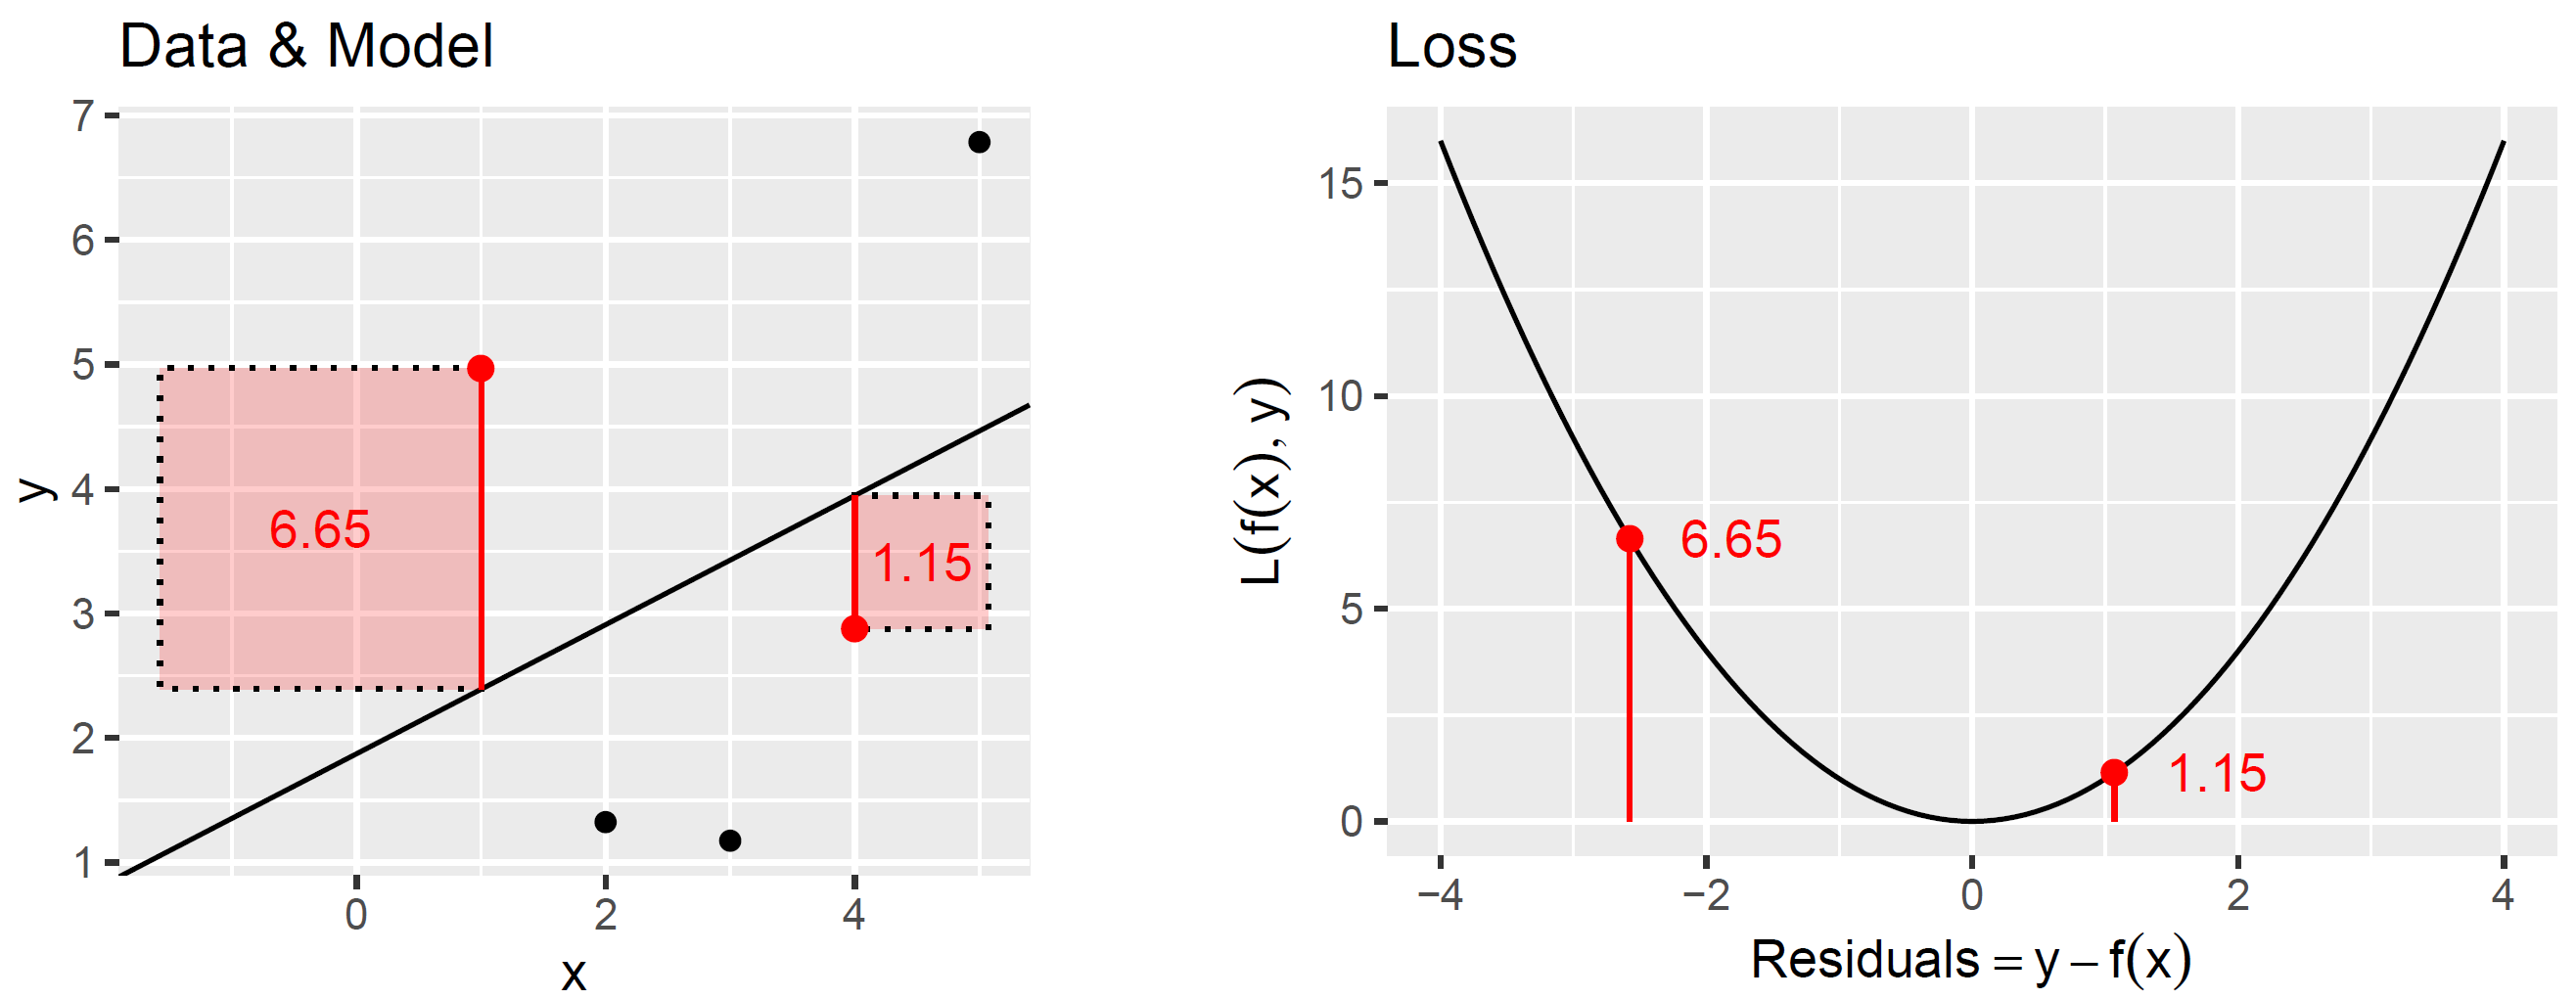
\includegraphics[width=1\columnwidth]{img/reg_loss.PNG}
								\textbf{Conditional entropy} of $Y$  given $X$ for $(X, Y) \sim p(x, y):$
								% 
								\vspace{-0.2cm}
								%
								\begin{small}  
									\begin{equation*}
										\begin{aligned}
											H(Y | X) &= \E_X[H(Y|X=x)] = \sum_{x \in \Xspace} p(x) H(Y | X=x) \\
											&=-\sum_{x \in \Xspace} p(x) \sum_{y \in \Yspace} p(y | x) \log p(y | x) 
											=-\sum_{x \in \Xspace} \sum_{y \in \Yspace} p(x, y) \log p(y | x)  
										\end{aligned}
									\end{equation*}
								\end{small}  
								%
								Chain rule for entropy:
								%
								$$H(X, Y)=H(X)+H(Y | X)$$
								%
								n-Variable version:
								$$H\left(X_{1}, X_{2}, \ldots, X_{n}\right)=\sumin H\left(X_{i} | X_{i-1}, \ldots, X_{1}\right)$$
								%
								Other properties:
								%
								\begin{itemize}
									\setlength{\itemindent}{+.3in}
										\item $H(X, X)       = H(X)  $
										\item $H(X | X)      = 0 $
										\item $H(X, Y | Z)   =H(X | Z)+H(Y | X, Z)$
										\item $H(X | Y) \leq H(X) $
										\item  If $H(X|Y) = 0$, then $X$ is a function of $Y$
								\end{itemize}
								%
								\textbf{Mutual information} between $X$ and $Y:$
								%
								\begin{equation*}
									\begin{aligned}
										I(X ; Y) &= \E_{p(x, y)} \left[ \log \frac{p(X, Y)}{p(X) p(Y)} \right] = \sum_{x \in \Xspace} \sum_{y \in \Yspace} p(x, y) \log \frac{p(x, y)}{p(x) p(y)} \\
										&= H(X)-H(X | Y)
									\end{aligned}
								\end{equation*}
								%
								Properties:
								\begin{itemize}
									\setlength{\itemindent}{+.3in}
										\item $ I(X ; Y) = H(X) - H(X | Y) $
											\item $I(X ; Y) = H(Y) - H(Y | X) $
											\item $I(X ; Y) = H(X) + H(Y) - H(X, Y)$
											\item $I(X ; Y) = I(Y ; X) $
											\item $I(X ; X) = H(X)$
											\item $ I(X;Y) \geq 0$, with equality if and only if $X$ and $Y$ are independent
								\end{itemize}
								%
								\textbf{Cross-entropy} of two distributions $p$ and $q$ on the same domain $\Xspace:$
								%
								$$ 
									H_q(p) = \sum_{x \in \Xspace} p(x) \log\left(\frac{1}{q(x)}\right) = - \sum_{x \in \Xspace} p(x) \log\left(q(x)\right) 
								$$
								%
								\textbf{Kullback-Leibler Divergence:}
								%
								$$ 
									D_{KL}(p \| q) = \E_p \left[\log \frac{p(X)}{q(X)}\right] = \sum_{x \in \Xspace} p(x) \cdot \log \frac{p(x)}{q(x)} 
								$$
								%
								Relationship:
								$$
									H_q(p) = H(p) + D_{KL}(p \| q)
								$$
							\end{myblock}



			  			}
					\end{minipage}
				\end{beamercolorbox}
			\end{column}
		\end{columns}

	\end{frame}
\end{document}



%-------------------------------------------------------------------------------
% Classification 
%------------------------------------------------------------------------------- 

%\begin{myblock}{Classification}
% 				    We want to assign new observations to known categories according to criteria learned from a training set.  
%             \vspace*{1ex}
%             

%$y \in \Yspace = \gset : $ categorical output variable (label)\\ 

%\textbf{Classification} usually means to construct $g$ \textbf{discriminant functions}:
  
%$f_1(\xv), \ldots, \fgx$, so that we choose our class as \\ $h(\xv) = \argmax_{k \in \gset} \fkx$ \\

%\textbf{Linear Classifier:} functions $\fkx$ can be specified as linear functions\\

% \hspace*{1ex}\textbf{Note: }All linear classifiers can represent non-linear decision boundaries \hspace*{1ex}in our original input space if we include derived features. For example: \hspace*{1ex}higher order interactions, polynomials or other transformations of x in \hspace*{1ex}the model.

%\textbf{Binary classification: }If only 2 classes ($\Yspace = \setzo$ or  $\Yspace = \setmp$) exist, we can use a single discriminant function $\fx = f_{1}(\xv) - f_{2}(\xv)$.  \\


% \textbf{Generative approach }models $\pdfxyk$, usually by making some assumptions about the structure of these distributions and employs the Bayes theorem: 
% $\pikx = \postk \propto \pdfxyk \pik$. \\ %It allows the computation of \hspace*{1ex}$\pikx$. \\
% \textbf{Examples}: Linear discriminant analysis (LDA), Quadratic discriminant analysis (QDA), Naive Bayes\\
% 
% \textbf{Discriminant approach }tries to optimize the discriminant functions directly, usually via empirical risk minimization:\\ 
% $ \fh = \argmin_{f \in \Hspace} \riske(f) = \argmin_{f \in \Hspace} \sumin \Lxyi.$\\
% \textbf{Examples}: Logistic/softmax regression, kNN


%\end{myblock}

%-------------------------------------------------------------------------------
% HRO - Components of Learning 
%-------------------------------------------------------------------------------          
%\begin{myblock}{Components of Learning}

%\textbf{Learning = Hypothesis space + Risk + Optimization} \\
%\phantom{\textbf{Learning}} \textbf{= }$ \Hspace + \risket + \argmin_{\thetav \in \Theta} 
%\risket$

% 
% \textbf{Learning &= Hypothesis space &+ Risk  &+ Optimization} \\
% &= $\Hspace &+ \risket &+ \argmin_{\thetav \in \Theta} \risket$
% 
% \textbf{Hypothesis space: } Defines (and restricts!) what kind of model $f$
% can be learned from the data.
% 
% Examples: linear functions, decision trees
% 
% \vspace*{0.5ex}
% 
% \textbf{Risk: } Quantifies how well a model performs on a given
% data set. This allows us to rank candidate models in order to choose the best one.
% 
% Examples: squared error, negative (log-)likelihood
% 
% \vspace*{0.5ex}
% 
% \textbf{Optimization: } Defines how to search for the best model, i.e., the model with the smallest {risk}, in the hypothesis space.
% 
% Examples: gradient descent, quadratic programming


%\end{myblock}
% End Third Column
%%%%%%%%%%%%%%%%%%%%%%%%%%%%%%%%%%%%%%%%%%%%%%%%%%%%%%%%%%%%%%%%%%%%%%%%%%%%%%%%